% Autor: Daniel Tatzel

\section{Sprachauswahl}

\subsection{Startseite}

Auf der Startseite kann die gewünschte Sprache über die entsprechende Flagge ausgewählt werden, siehe Grafik \ref{fig:startseite}.

\begin{figure}[!htbp]
 \centering
 
\includegraphics[width=1\textwidth]{../Screenshots/startseite}
 \label{fig:startseite}
 \caption{Die erste Seite}
\end{figure}

\newpage

\subsection{Folgeseiten}

Hat man sich bei der Sprachauswahl vertan oder möchte die Inhalte in der jeweils anderen Sprache lesen, so kann durch ein Click auf die Flagge im Menü die Sprache gewechselt werde, siehe
Auf der Startseite kann die gewünschte Sprache über die entsprechende Flagge ausgewählt werden, siehe Grafik \ref{fig:startseite}.

\begin{figure}[!htbp]
 \centering
 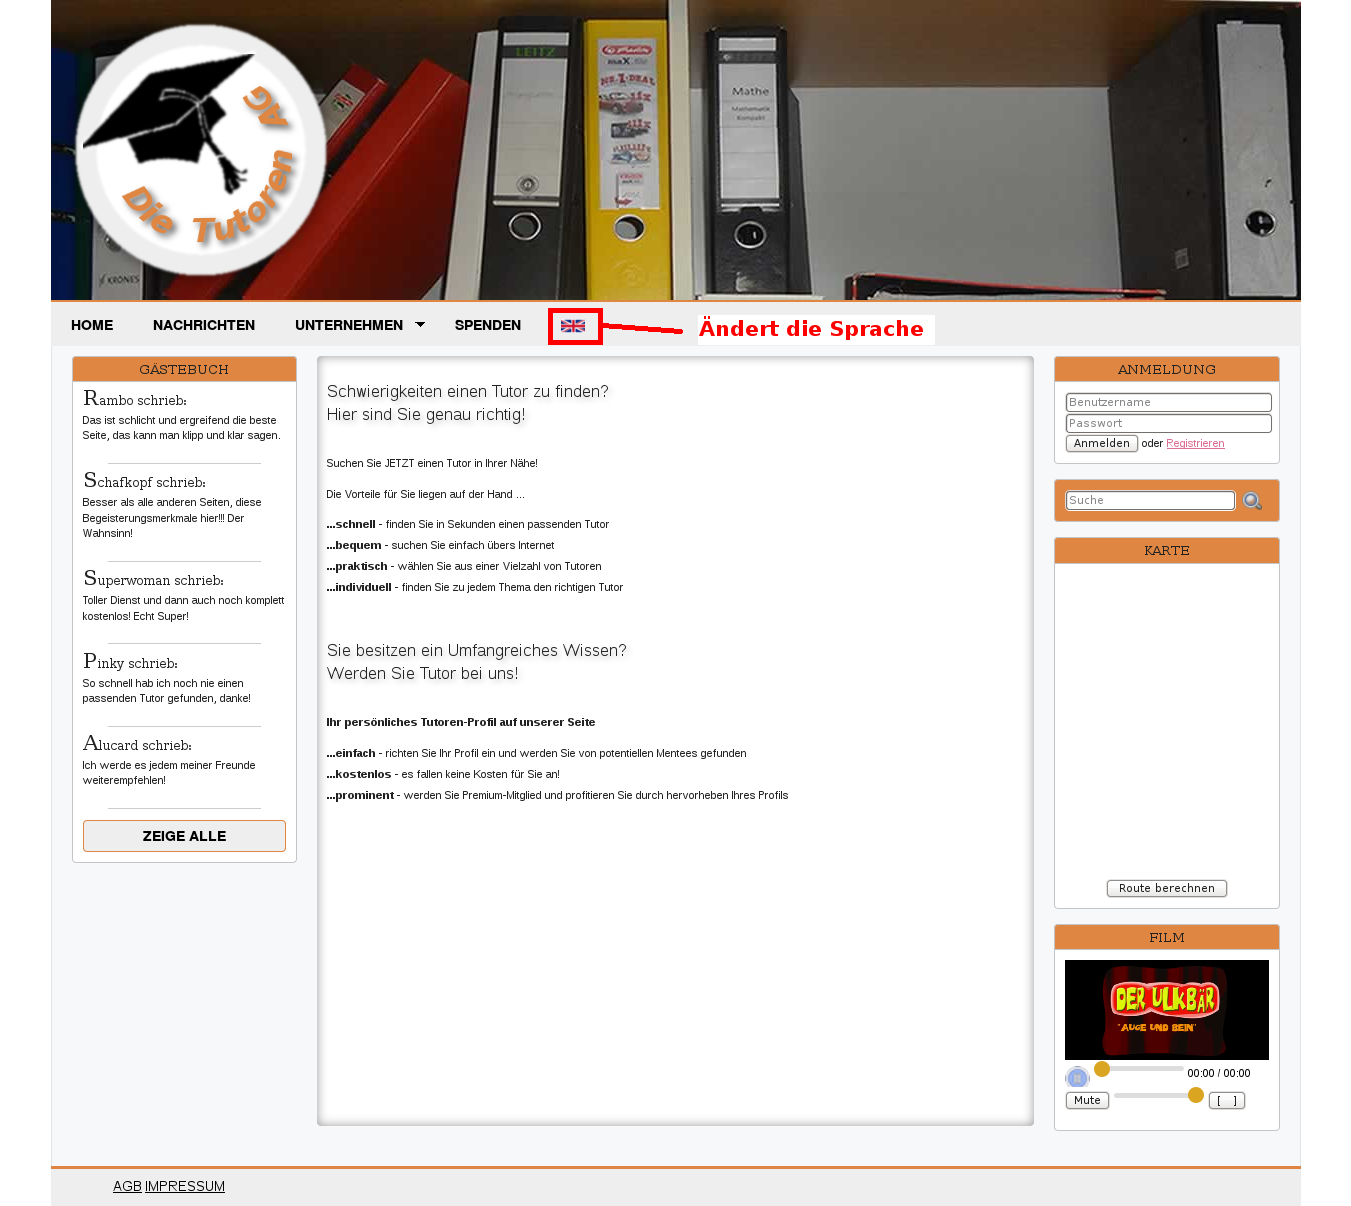
\includegraphics[width=1\textwidth]{../Screenshots/de/sprachauswahl}
 \label{fig:sprachauswahl}
 \caption{Sprachauswahl auf den Folgeseiten}
\end{figure}
